\scanpage{26}
% Folio d'archive : 25. Circulaire imprimée et dactylographiée, tampons et signature.
REPUBLIQUE FRANÇAISE

Ministère de la recherche et de l'industrie
\figure{\begin{tikzpicture}\draw (0,0)--(12,0);\end{tikzpicture}}
Mission scientifique et technique\hfill Paris, le\quad 30 Mars 1983
\figure{\begin{tikzpicture}\draw (0,0)--(12,0);\end{tikzpicture}}

1 rue Descartes\\
75231 Paris Cedex 05\\
Tél. 634'33 33 / 634 35 35\\
Telex MRIACR 204 643 F

Réf.

% Tampon de réception, à droite du bloc d'adresse.
\figure{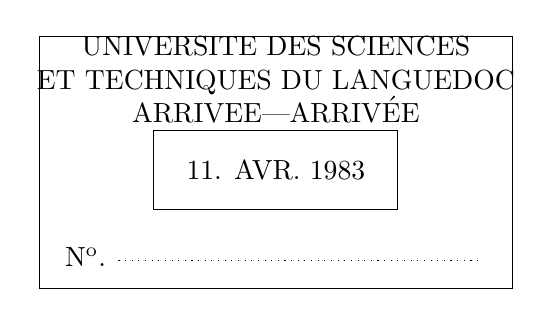
\begin{tikzpicture}
\draw (0,0) rectangle (6,3.2);
\node[align=center] at (3,2.65) {UNIVERSITE DES SCIENCES\\ET TECHNIQUES DU LANGUEDOC\\\unsure{ARRIVEE|ARRIVÉE}};
\draw (1.45,1) rectangle (4.55,2);
\node at (3,1.5) {11. AVR. 1983};
\node[anchor=west] at (.2,.4) {N\textsuperscript{o}.};
\draw[dotted] (1,.35)--(5.6,.35);
\end{tikzpicture}}

Messieurs, Mesdames les Directeurs de Formation de Recherche,

Le développement des techniques au service de la recherche dans
le domaine des Sciences de la Vie nous amène à nous préoccuper de la
planification de l'équipement en matériels semi-lourds de nos laboratoires
(nous entendons par matériels semi-lourds des appareils dont le prix
d'achat est compris entre 0,5 et 5 millions de francs).

Nous désirons tout d'abord faire une mise au point sur l'état actuel
du parc des appareils semi-lourds et de leur ancienneté, deuxièmement
connaitre les besoins actuels et futurs pour ces types d'appareils, dont
la liste non exhaustive est ci-jointe.

Pour chaque type d'appareils existant dans votre laboratoire,
veuillez nous préciser la date d'achat et la source du financement de cet
appareil et d'autre part veuillez nous faire savoir quels sont vos
besoins actuels et vos besoins prévisibles pour les prochaines années
(84-89) concernant ces équipements semi-lourds.

Une fiche réponse est jointe à cette lettre, elle devrait nous être
retournée si possible par retour du courrier.

L'ensemble des réponses seront dépouillées avant la fin avril 1983
et vous serez personnellement informé des résultats de l'enquête et des
prospectives.

Je vous remercie d'avance pour votre diligente collaboration, et
vous prie de croire, Cher Collègue, à mes sentiments les meilleurs.

% Signature manuscrite, puis nom dactylographié.
\figure{
\begin{tikzpicture}
\node[font=\itshape] at (2,.6) {D. Pantaloni};
\draw (0,.2)..controls (1,.1) and (.8,.9)..(.3,1)..controls (.25,.6) and (.45,.2)..(.45,.35);
\draw (1.3,.35)..controls (1.1,1.3) and (2,1.45)..(1.8,1.1)..controls (1.7,1) and (1.3,1)..(1.4,.2);
\end{tikzpicture}}
\begin{flushright}D. Pantaloni\end{flushright}

% Mention de transmission encadrée, en bas à gauche.
\figure{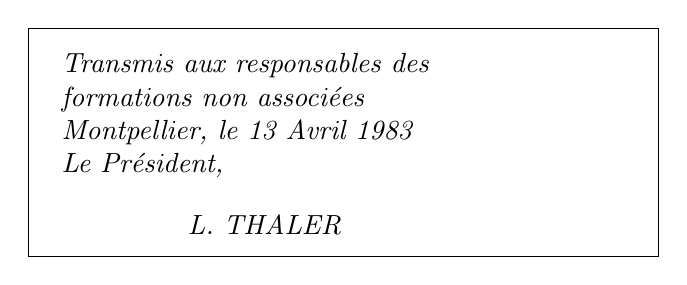
\begin{tikzpicture}
\draw (0,0) rectangle (8,2.9);
\node[anchor=north west,align=left,font=\itshape] at (.3,2.7)
{Transmis aux responsables des\\formations non associées\\Montpellier, le 13 Avril 1983\\Le Président,};
\node[font=\itshape] at (3,.4) {L. THALER};
\end{tikzpicture}}
% Tampon circulaire chevauchant le cadre et la première ligne du P.S.
\figure{
\begin{tikzpicture}
\draw (0,0) circle (1.7);\draw (0,0) circle (1.25);
\node[align=center] at (0,.95) {ACADEMIE DE MONTPELLIER};
\node[align=center,font=\small] at (0,-.15)
{UNIVERSITE\\DES SCIENCES ET\\TECHNIQUES DU\\LANGUEDOC};
\fill (0,-1.45) circle (2pt);
\end{tikzpicture}}

P.S. Une seconde feuille réponse est jointe à cette lettre afin que
vous puissiez la diffuser éventuellement auprès de collègues
universitaires qui n'appartiendraient pas à une formation de recherche
du C.N.R.S. où de l'I.N.S.E.R.M.
